\section{Creating a new ESCRIBA project}

After installing all project dependencies, you are ready to download and use
\ESCRIBA. Because this tool is simply a \LaTeX template it does not require from
an installation but from a cookiecutter call. Hence, start a new \ESCRIBA
project by running the command from figure \ref{fig:installing_escriba}:


\begin{figure}[h]
  \centering
  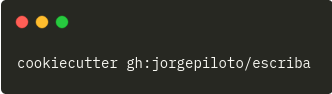
\includegraphics[scale=0.5]{static/install_escriba.png}
  \caption{The command to create a new ESCRIBA project.}
  \label{fig:installing_escriba}
\end{figure}

Previous command will ask you to input some parameters such us the name of your
project, the title of your work, author, location and date among others. These
parameters might become more complex as the project evolves.
